\chapter{Manual}
\label{MAN}

This manual will explain the basic use of the map, as well as its
advances features. The images are from Mac OS X and might look different on other
operating systems.

\section{Navigation}
\label{MAN-N}
At startup, the entire country of Denmark is shown. Now, we can move around the
map with both the direction buttons in the top left corner, and the arrow keys.
To move west, click the button
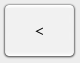
\includegraphics[height=1.3em]{images/westbutton.png} or press the left arrow
key. This goes for all four directions.

\begin{figure}[h!]
\centering
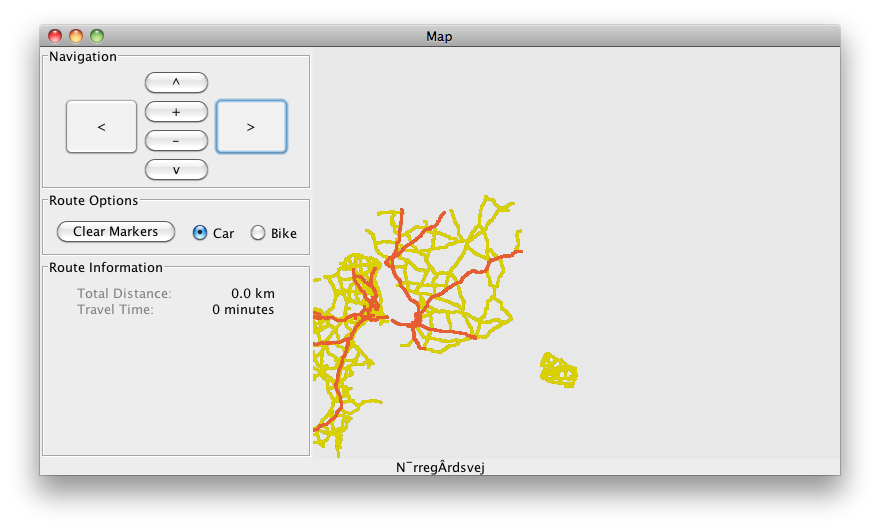
\includegraphics[width=1\linewidth]{images/man-move.png}
\caption{Moving the map}
\label{MAN-Z-COP}
\end{figure}

\section{Zoom}
\label{MAN-Z}
To zoom-in on the map, click the

\includegraphics[height=1.5em]{images/zoominbutton.png} button in the navigation
panel.

To zoom-in on a specific area, click the mouse and drag a rectangle around that
area on the map. A blue transparent rectangle will show you what you have
selected. To zoom-in, release the mouse-button.

For example, if you want to zoom-in on Copenhagen,
click the upper left corner of the city, and drag the cursor to the lower right
corner.

\begin{figure}[h!]
\centering
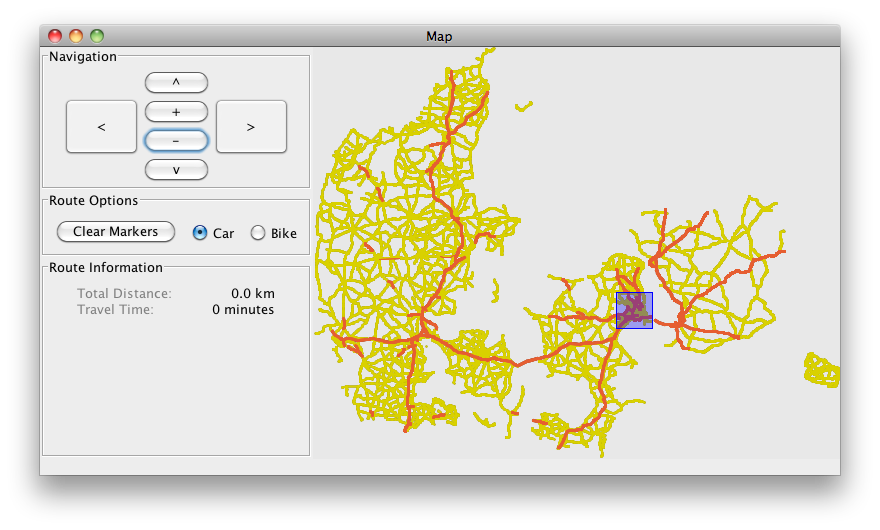
\includegraphics[width=1\linewidth]{images/man-copenhagen.png}
\caption{Zooming in on Copenhagen}
\label{MAN-Z-COP}
\end{figure}

To zoom-out of the map, click the
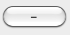
\includegraphics[height=1.5em]{images/zoomoutbutton.png} button. To return to
the startup view (showing the entire map of Denmark) press the \class{ESC} button.

\section{Route find}
\label{MAN-RF}
To find a route from one point to another, you must specify a start and an end
location. Click anywhere on the map to choose your start location. A light blue
marker will appear, containing the number ``1''. To choose your end location,
click at another location. A marker containing the number ``2'' will appear. The
best route from 1 to 2 will be calculated, and shown on the map as a blue path.
To extend your route with more markers, you can click at a new location on the
map. You can repeat this an unlimited amount of times. You can delete one of
your markers by clicking at its root. To delete all marker, click the button
'clear markers' or press \class{c} on the keyboard.

\begin{figure}[h!]
\centering
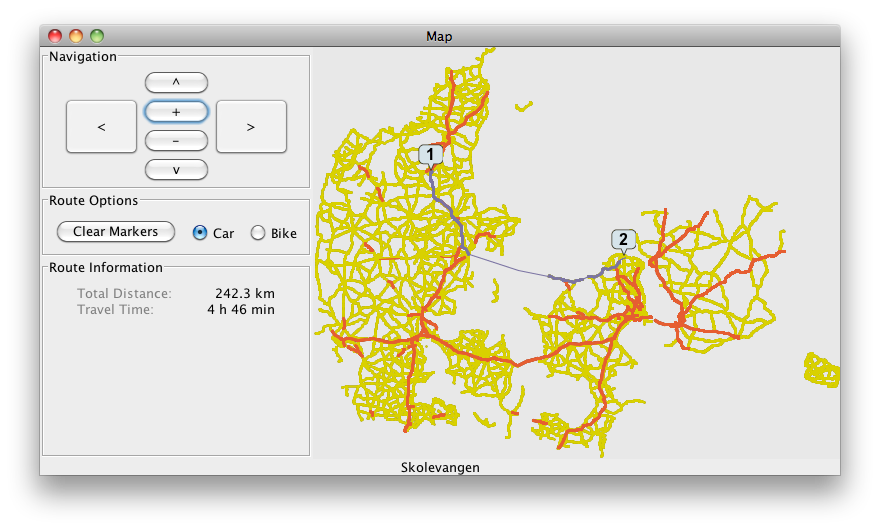
\includegraphics[width=1\linewidth]{images/man-route.png}
\caption{A route from 1 to 2 has been calculated}
\label{MAN-RF-IMG}
\end{figure}

\section{Bike/car}
\label{MAN-BC}
When calculating routes, it is important to specify which form of
transportation you wish to use. Choose your preferred style of transportation by
selecting the corresponding radio button.

\begin{figure}[h!]
\centering
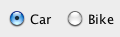
\includegraphics[height=2em]{images/radiobuttons.png}
\caption{The radiobuttons}
\label{MAN-BC-IMG}
\end{figure}

The form of transportation you use will have big influence on what route is
calculated. If the car option is chosen, the route will be optimized for car
transportation. If the bicycle option is chosen, the route will be optimized for
bicycling.

\section{Resize}
\label{MAN-RS}
To resize the map, drag the window as you would with any other application. The
map will automatic adjust to the new size of the window.
\begin{figure}[h!]
\centering
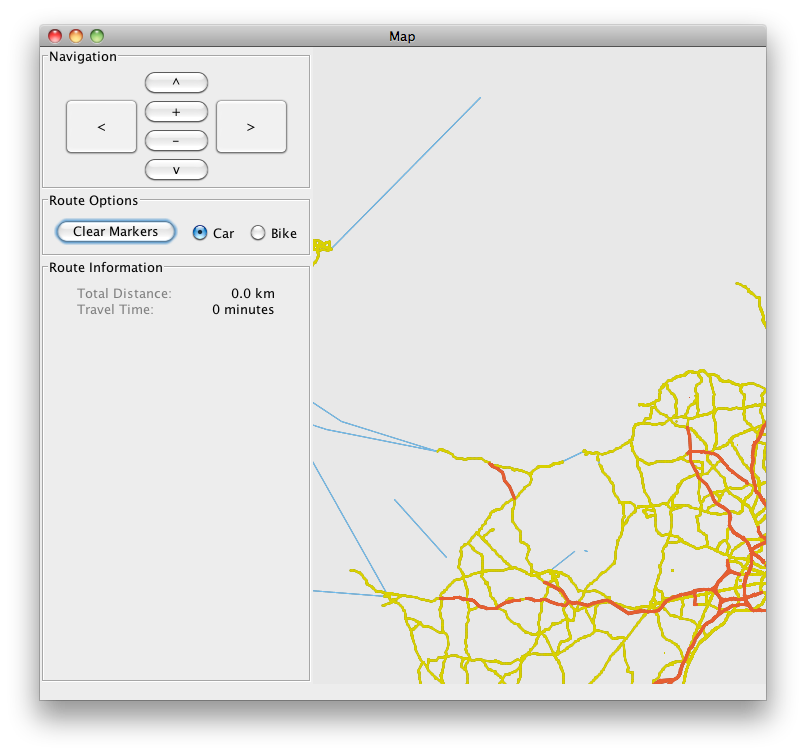
\includegraphics[width=1\linewidth]{images/man-resize.png}
\caption{The map has been resized}
\label{man-radio}
\end{figure}